%%%%%%%%%%%%%%%%%%%%%%%%%%%%%%%%%%%%%%%%%
% Beamer Presentation
% LaTeX Template
% Version 1.0 (10/11/12)
%
% This template has been downloaded from:
% http://www.LaTeXTemplates.com
%
% License:
% CC BY-NC-SA 3.0 (http://creativecommons.org/licenses/by-nc-sa/3.0/)
%
%%%%%%%%%%%%%%%%%%%%%%%%%%%%%%%%%%%%%%%%%

%----------------------------------------------------------------------------------------
%	PACKAGES AND THEMES
%----------------------------------------------------------------------------------------

\documentclass[aspectratio=32]{beamer}
\usefonttheme[onlymath]{serif}


\mode<presentation> {

% The Beamer class comes with a number of default slide themes
% which change the colors and layouts of slides. Below this is a list
% of all the themes, uncomment each in turn to see what they look like.

\usetheme{default}
%\usetheme{AnnArbor}
%\usetheme{Antibes}
%\usetheme{Bergen}
%\usetheme{Berkeley}
%\usetheme{Berlin}
%\usetheme{Boadilla}
%\usetheme{CambridgeUS}
%\usetheme{Copenhagen}
%\usetheme{Darmstadt}
%\usetheme{Dresden}
%\usetheme{Frankfurt}
%\usetheme{Goettingen}
%\usetheme{Hannover}
%\usetheme{Ilmenau}
%\usetheme{JuanLesPins}
%\usetheme{Luebeck}
%\usetheme{Malmoe}
%\usetheme{Marburg}
%\usetheme{Montpellier}
%\usetheme{PaloAlto}
%\usetheme{Pittsburgh}
%\usetheme{Rochester}
%\usetheme{Singapore}
%\usetheme{Szeged}
%\usetheme{Warsaw}

% As well as themes, the Beamer class has a number of color themes
% for any slide theme. Uncomment each of these in turn to see how it
% changes the colors of your current slide theme.

%\usecolortheme{albatross}
%\usecolortheme{beaver}
\usecolortheme{spruce}
%\usecolortheme{beetle}
%\usecolortheme{crane}
%\usecolortheme{dolphin}
%\usecolortheme{dove}
%\usecolortheme{fly}
%\usecolortheme{lily}
%\usecolortheme{orchid}
%\usecolortheme{rose}
%\usecolortheme{seagull}
%\usecolortheme{seahorse}
%\usecolortheme{whale}
%\usecolortheme{wolverine}

%\setbeamertemplate{footline} % To remove the footer line in all slides uncomment this line
%\setbeamertemplate{footline}[page number] % To replace the footer line in all slides with a simple slide count uncomment this line

%\setbeamertemplate{navigation symbols}{} % To remove the navigation symbols from the bottom of all slides uncomment this line
}


\usepackage{graphicx} % Allows including images
\usepackage{booktabs} % Allows the use of \toprule, \midrule and \bottomrule in tables
\usepackage{verbatim}
\usepackage{colortbl}

\usepackage{mathtools} 
\usepackage{amssymb}
\usepackage{mathrsfs}
\usepackage{amsmath}
\usepackage{bm}

\usepackage{ragged2e}
\usepackage{etoolbox}
\usepackage{lipsum}

\usepackage{siunitx,booktabs}
\usepackage{pifont}
\usepackage{array}
\usepackage{tabu,booktabs}
\usepackage{tikz,threeparttable}
\usetikzlibrary{arrows,shapes}

\setbeamertemplate{enumerate items}[circle]
\usepackage{tikz}

\newcommand\mynum[1]{
  \usebeamercolor{enumerate item}
  \tikzset{beameritem/.style={circle,inner sep=0,minimum size=2ex,text=enumerate item.bg,fill=enumerate item.fg,font=\footnotesize}}%
  \tikz[baseline=(n.base)]\node(n)[beameritem]{#1};
}

\newcommand\mynumm[1]{
  \usebeamercolor{enumerate item}
  \tikzset{beameritem/.style={rectangle,inner sep=0,minimum size=2ex,text=enumerate item.bg,fill=enumerate item.fg,font=\footnotesize}}%
  \tikz[baseline=(n.base)]\node(n)[beameritem]{#1};
}
% COLUMN TYPES
\newcolumntype{L}[1]{>{\raggedright\let\newline\\\arraybackslash\hspace{0pt}}m{#1}}
\newcolumntype{C}{>{\centering\arraybackslash}p{5.2em}}
\newcolumntype{D}{>{\centering\arraybackslash}p{5em}}
\newcolumntype{G}{>{\centering\arraybackslash}p{6em}}
\newcolumntype{R}[1]{>{\raggedleft\let\newline\\\arraybackslash\hspace{0pt}}m{#1}}



\def\Put(#1,#2)#3{\leavevmode\makebox(0,0){\put(#1,#2){#3}}}

\setbeamertemplate{footline}[frame number]

\AtBeginSection[]{
  \begin{frame}
  \vfill
  \centering
  \begin{beamercolorbox}[sep=8pt,center,shadow=true,rounded=true]{title}
    \usebeamerfont{title}\insertsectionhead\par%
  \end{beamercolorbox}
  \vfill
  \end{frame}
}

%----------------------------------------------------------------------------------------
%	TITLE PAGE
%----------------------------------------------------------------------------------------

\title{Public Housing Spillovers: \\Evidence from South Africa} % The short title appears at the bottom of every slide, the full title is only on the title page

\author{\\Ben Bradlow (Harvard University) \\ Stefano Polloni (MapDwell)\\ Will Violette (Federal Trade Commission) \\ william.j.violette@gmail.com \\[2em] Any opinions expressed herein are those of the authors
and do not necessarily represent the views of the
Federal Trade Commission.} 


 % Your institution as it will appear on the bottom of every slide, may be shorthand to save space

\date{October 2020} %\today} % Date, can be changed to a custom date

\begin{document}

\beamertemplatenavigationsymbolsempty

\begin{frame}
\titlepage % Print the title page as the first slide
\end{frame}

%\begin{frame}
%\frametitle{Overview} % Table of contents slide, comment this block out to remove it
%\tableofcontents % Throughout your presentation, if you choose to use \section{} and \subsection{} commands, these will automatically be printed on this slide as an overview of your presentation
%\end{frame}

%----------------------------------------------------------------------------------------
%	PRESENTATION SLIDES
%----------------------------------------------------------------------------------------
%------------------------------------------------

\begin{frame}
\frametitle{Public Housing and Development}
\centering
% In developing countries, 30\% of urban pop live in slums (UN, 2015)

\begin{itemize}
  \item In developing countries, 30\% of urban pop. live in informal housing [UN, 2015]
  \vspace{2mm}
  \item In Africa, governments have built $\sim$5.4 mil. houses often replacing slums ($\sim$3 mil. in South Africa)
  \vspace{2mm}
  \item Place-Based Policy?
  \begin{itemize}
  \item Housing projects may improve congestion, sanitation, and investment; or they may invite new slum growth (ie. backyard housing [Brueckner et al., 2019])
\end{itemize}
  \vspace{2mm}

\end{itemize}

\end{frame}

% place-based policy: slow down, make it clear



% %------------------------------------------------

\begin{frame}
\frametitle{This paper}
\centering

\begin{itemize}
    \item Asks how housing projects in Johannesburg affect areas \textit{within} as well as \textit{nearby} project footprints
  \vspace{2mm}
  \item Compares changes in outcomes by exposure to 166 constructed projects and 140 planned, but unconstructed projects
  \begin{itemize}
    \item Measures exposure as neighborhood overlap with project footprints
  \end{itemize}
  \vspace{2mm}

  \item Finds that both formal + informal housing grow both within + nearby footprints
  \vspace{2mm}

  \item Better houses, improved public goods, and more local firms help explain positive spillovers
   
\end{itemize}

% do indeed confirm that this is the policy, formal outside is probably new housing!!!

\end{frame}


% \begin{frame}
% \frametitle{Public Housing in South Africa}
% % \centering
% \centering
% \begin{itemize}
%   \item Large 
%     \vspace{2mm}
%   \item 
%     \vspace{2mm}
%   \item 
% \end{itemize}
% \end{frame}



{ % all template changes are local to this group.
    \setbeamertemplate{navigation symbols}{}
    \begin{frame}<article:0>[plain]
        \begin{tikzpicture}[remember picture,overlay]
            \node[at=(current page.center)] {
                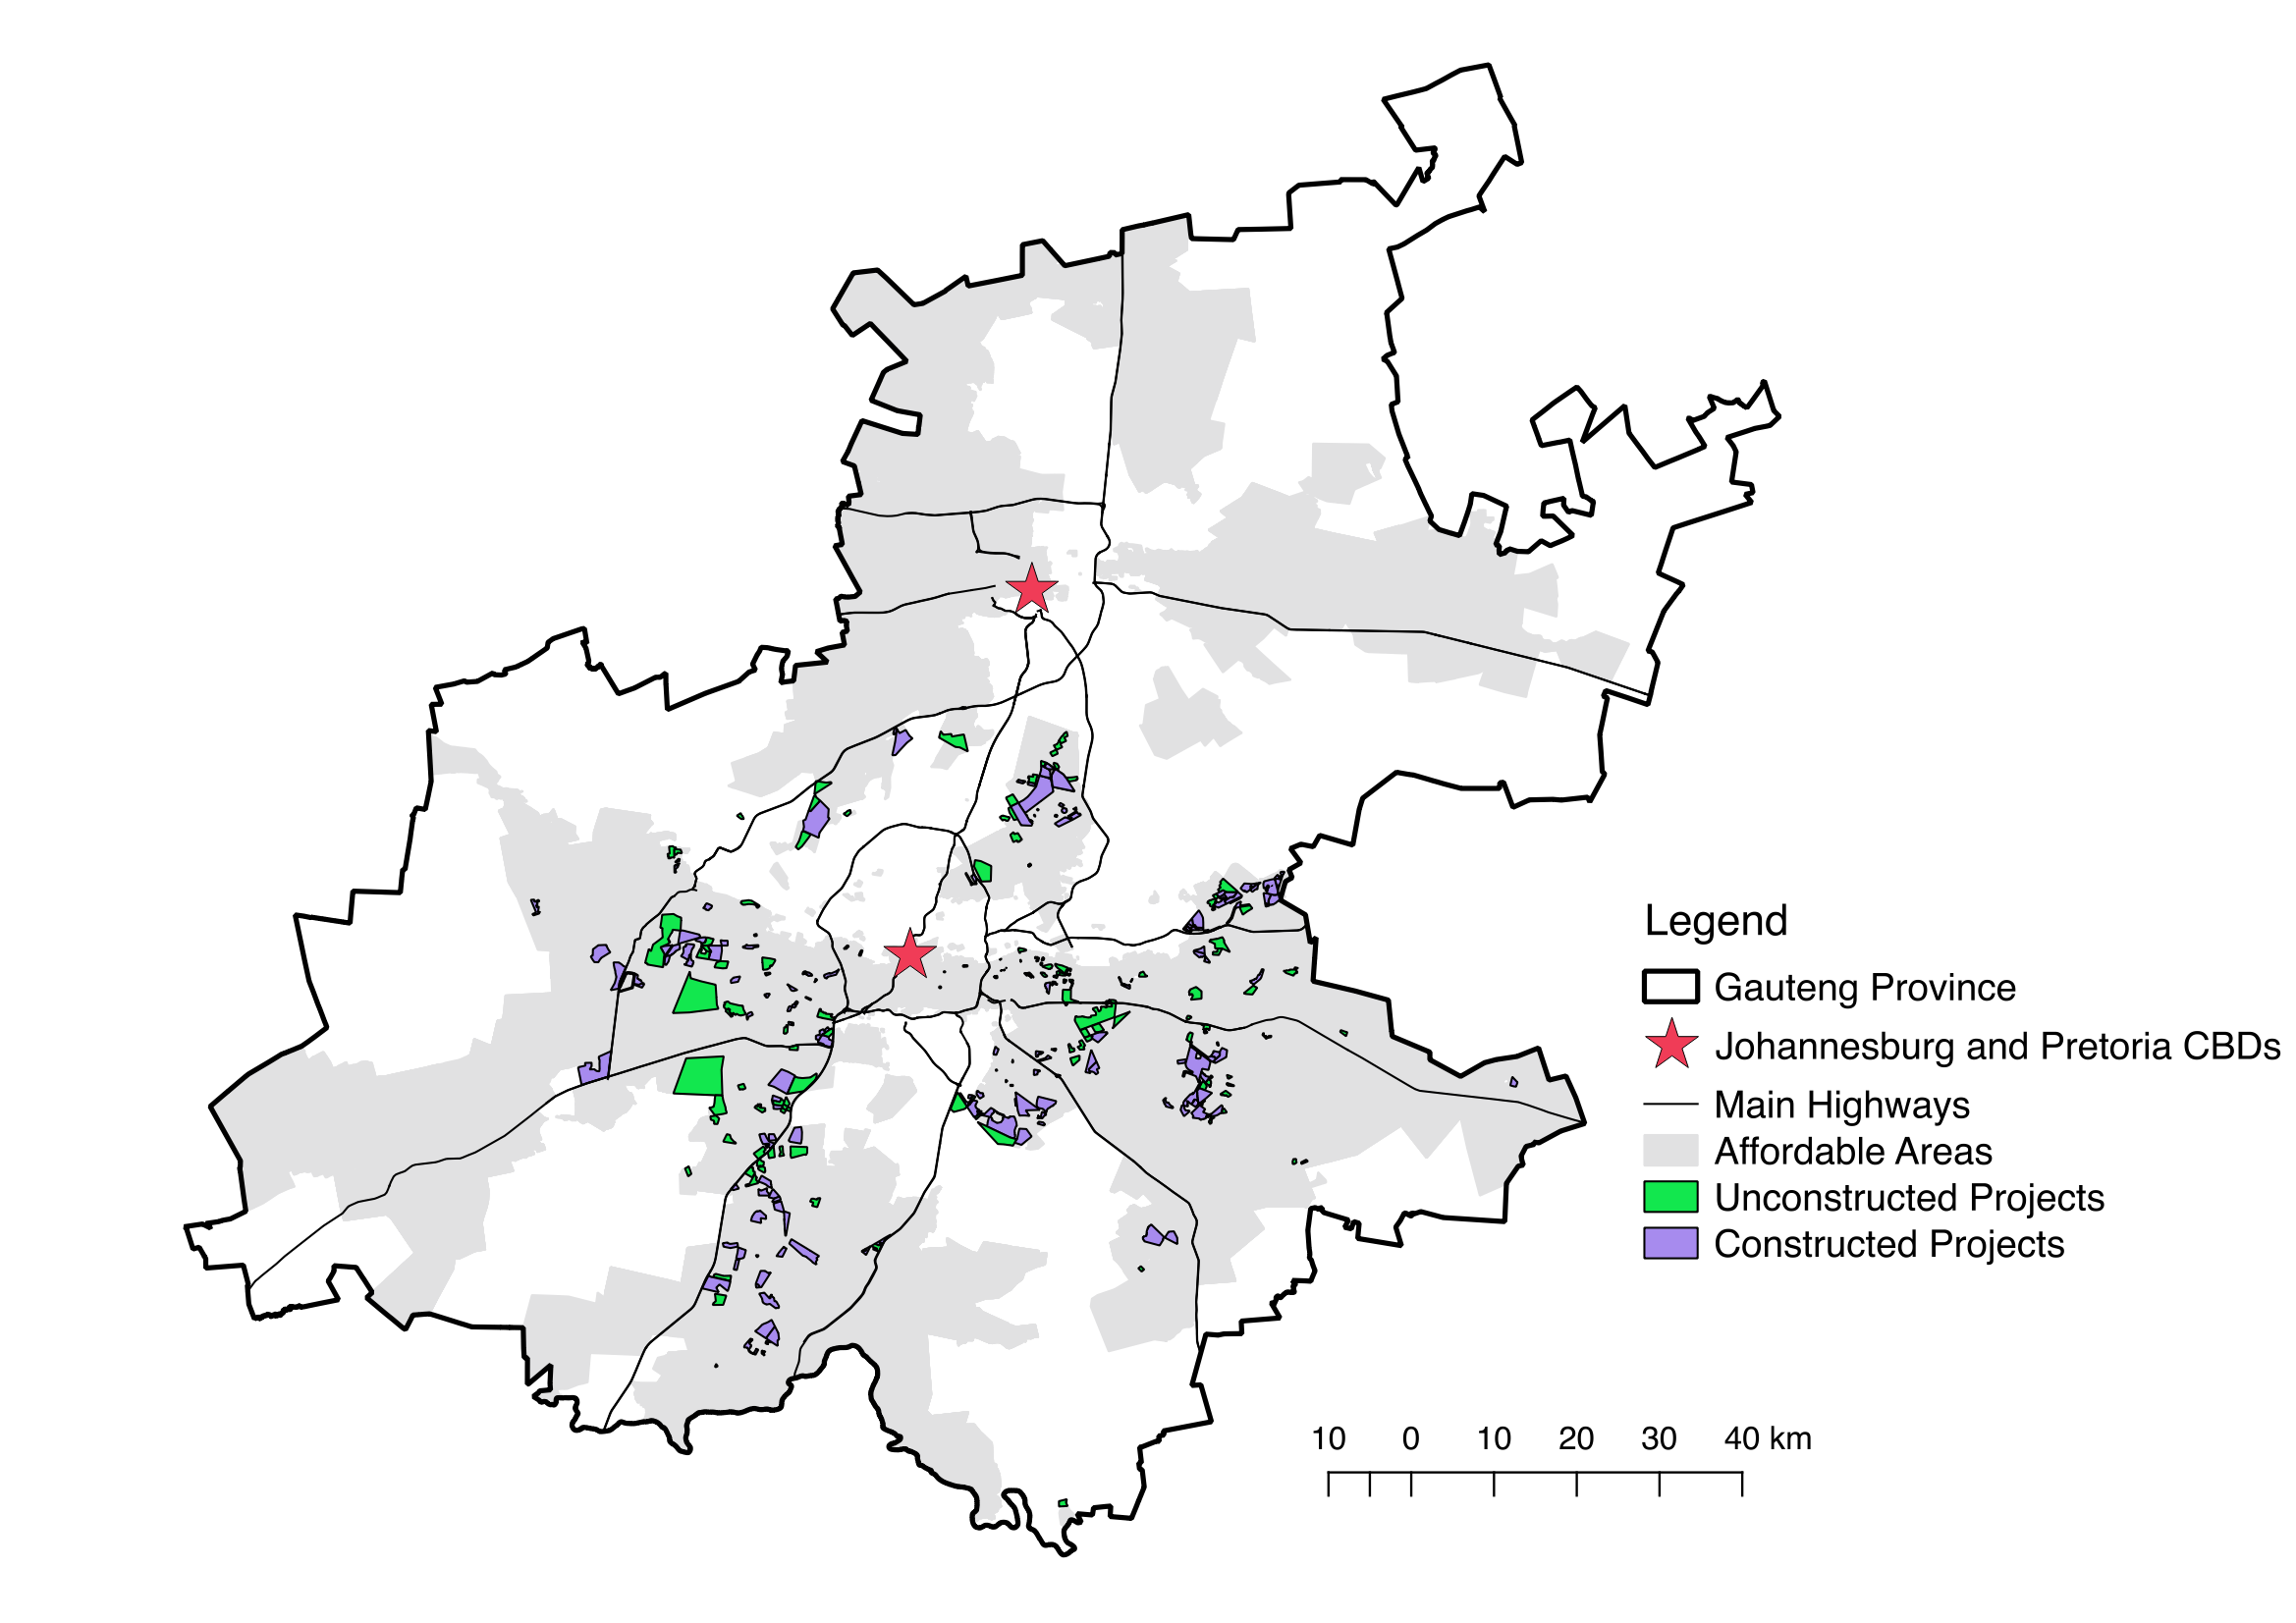
\includegraphics[keepaspectratio,
                                 width=\paperwidth,
                                 height=\paperheight]{figures/projmap_1.png}
            };
        \end{tikzpicture}
     \end{frame}
}

% gauteng greater MSA of joburg
% more formal about the datasource : GCRO from urban planners



{ % all template changes are local to this group.
    \setbeamertemplate{navigation symbols}{}
    \begin{frame}<article:0>[plain]
        \begin{tikzpicture}[remember picture,overlay]
            \node[at=(current page.center)] {
                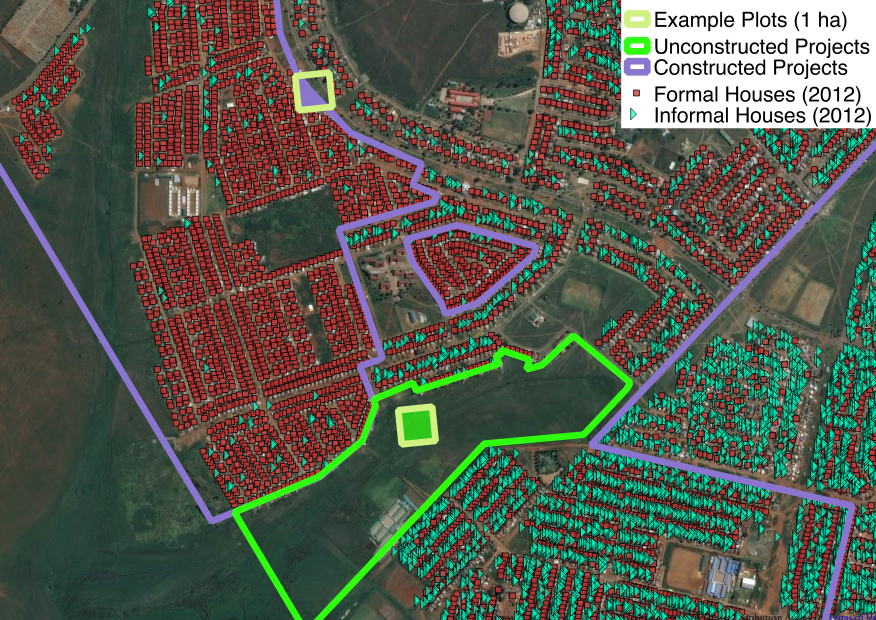
\includegraphics[keepaspectratio,
                                 width=\paperwidth,
                                 height=\paperheight]{figures/hm_proj_75.png}
            };
        \end{tikzpicture}
     \end{frame}
}


{ % all template changes are local to this group.
    \setbeamertemplate{navigation symbols}{}
    \begin{frame}<article:0>[plain]
        \begin{tikzpicture}[remember picture,overlay]
            \node[at=(current page.center)] {
                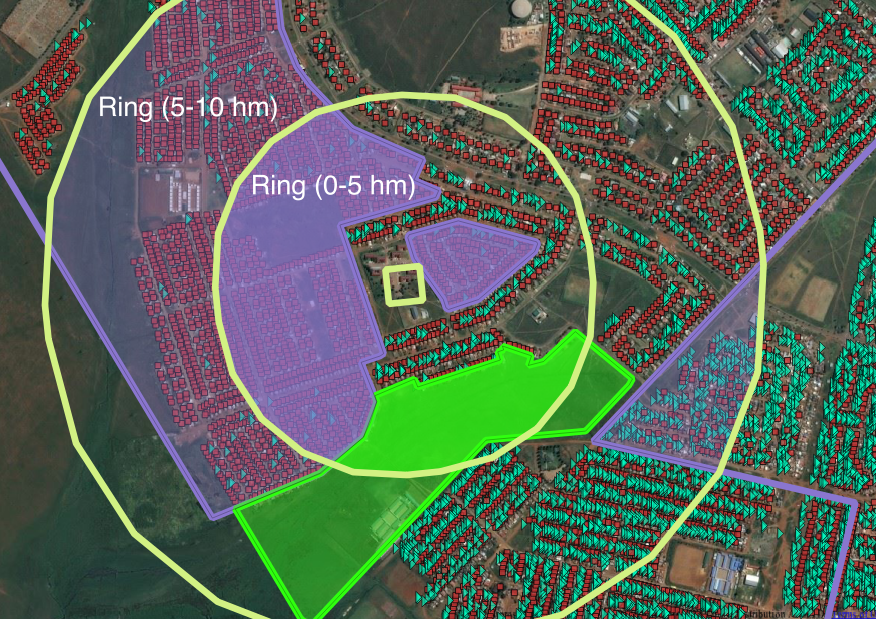
\includegraphics[keepaspectratio,
                                 width=\paperwidth,
                                 height=\paperheight]{figures/hm_spill_75.png}
            };
        \end{tikzpicture}
     \end{frame}
}




\begin{frame}
\frametitle{Estimating Direct and Spillover Effects}

\centering

\begin{align*}
\text{Direct}_{it} \,=\, &( \alpha_0 \, +  \, \alpha_1 \textsc{\small Post}_{t}) \, \times \, \text{Area}\big(\textsc{Plot}_i  \cap  \textsc{Proj.}\big) \, + \\[.5em]
&( \alpha_2 \, +  \, \alpha_3 \textsc{\small Post}_{t})  \, \times \, \text{Area}\big(\textsc{Plot}_i \cap \textsc{Con. Proj.}\big)
\end{align*}

\begin{align*}
\text{Spillover}_{it} \,=\, &\sum_{k=1}^{8} \, (\beta_{0}^{k} \,+\, \beta_{1}^{k} \textsc{\small Post}_{t})  \, \times \, \text{Area}\big(\textsc{Ring}_i^{k}  \cap  \textsc{Proj.}\big) \, + \\[.5em]
&\hspace{1.7em}(\beta_{2}^{k} \,+\, \beta_{3}^{k} \textsc{\small Post}_{t})  \, \times \,\text{Area}\big(\textsc{Ring}_i^{k}  \cap \textsc{Con. Proj.}\big)
\end{align*}


% \begin{align}
% \quad y_{it}  =\,& P_i \times \, \text{Direct}_{it} \, + \, (1- P_i) \times \, \text{Spillover}_{it} \,+\, \gamma_0 \,+\, \gamma_1 \, \textsc{Post}_t + \varepsilon_{it} \\[.5em]
% P_i =\,& \mathbbm{1}\Big\{\text{Area}\big(\textsc{Plot}_i  \cap  \textsc{Proj.}\big)>0\Big \}\,
% \end{align}

\end{frame}



\begin{frame}
\frametitle{Estimating Direct and Spillover Effects}

\centering

% \begin{align*}
% \text{Direct}_{it} \,=\, &( \alpha_0 \, +  \, \alpha_1 \textsc{\small Post}_{t}) \, \times \, \text{Area}\big(\textsc{Plot}_i  \cap  \textsc{Proj.}\big) \, + \\[.5em]
% &( \alpha_2 \, +  \, \alpha_3 \textsc{\small Post}_{t})  \, \times \, \text{Area}\big(\textsc{Plot}_i \cap \textsc{Con. Proj.}\big)
% \end{align*}

% \begin{align*}
% \text{Spillover}_{it} \,=\, &\sum_{k=1}^{K} \, (\beta_{0}^{k} \,+\, \beta_{1}^{k} \textsc{\small Post}_{t})  \, \times \, \text{Area}\big(\textsc{Ring}_i^{k}  \cap  \textsc{Proj.}\big) \, + \\[.5em]
% &\hspace{1.7em}(\beta_{2}^{k} \,+\, \beta_{3}^{k} \textsc{\small Post}_{t})  \, \times \,\text{Area}\big(\textsc{Ring}_i^{k}  \cap \textsc{Con. Proj.}\big)
% \end{align*}

\begin{align*}
\quad y_{it}  =\,& \, \text{Direct}_{it} \, + \, (1- P_i)  \, \text{Spillover}_{it} \,+\, \gamma_0 \,+\, \gamma_1 \, \textsc{Post}_t + \varepsilon_{it} \\[.5em]
\text{Where} & \\
P_i =\,& 1\Big\{\text{Area}\big(\textsc{Plot}_i  \cap  \textsc{Proj.}\big)>0\Big \}\,
\end{align*}

\begin{itemize}
\item Identification requires assuming parallel trends between exposure to constructed projects and exposure to planned, but unconstructed projects
\end{itemize}
\end{frame}



\begin{frame}
\frametitle{Data}

\centering
\begin{itemize}
\item Aerial building counts 2001/2012 per 1 ha plot
  \begin{itemize}
    \item Formal Houses, Informal Houses, Backyard Houses
    \item Water Utility Buildings, Electricity Utility Buildings, Health Centers, Schools, Businesses, Informal Businesses
  \end{itemize}
  \vspace{2mm}
\item Population/housing census in 2001/2011 overlapping 1 ha plots
  \begin{itemize}
    \item Population, Total Rooms, Own house, Electric Lighting, Flush Toilet, Piped Water Inside, Employment, Log HH Income
  \end{itemize}
    \vspace{2mm}
\item Deeds records of formal property transactions 2001-2011 overlapping 1 ha plots
  \begin{itemize}
    \item Count Transactions, Prices
  \end{itemize}
    \vspace{2mm}
\vspace{5mm}
\item Limitation: constructed project footprints have 4x more housing and 3x more population than unconstructed projects at baseline
\item Requires a strong parallel trends assumption
\end{itemize}



\end{frame}


\begin{frame}
\frametitle{Population and Housing Results}

\centering

\resizebox{1\linewidth}{!}{
\begin{tabular}{lCCCCC}
\toprule
                    % &(1)&(2)&(3)&(4)&(5)\\[.5em] 
                    &People                   &      Houses                   &Formal Houses                   &Informal Houses                   &Informal Backyard Houses \\ \midrule \\[-.6em]                   
Post $\times$ Constructed proj \\
overlap with: \\[1em] 
\hspace{1.5em}Plot footprint&      25.737\textsuperscript{a}&       9.102\textsuperscript{a}&       6.629\textsuperscript{a}&       2.473\textsuperscript{b}&       6.648\textsuperscript{a}\\
                    &     (4.630)                   &     (1.544)                   &     (0.812)                   &     (1.044)                   &     (1.157)                   \\[.5em]
\hspace{1.5em}Plot neighborhood &       0.213\textsuperscript{a}&       0.070\textsuperscript{a}&       0.023\textsuperscript{b}&       0.047\textsuperscript{b}&       0.037\textsuperscript{a}\\
\hspace{1.5em} (0-5 hm ring)                   &     (0.075)                   &     (0.023)                   &     (0.011)                   &     (0.019)                   &     (0.013)                   \\[.5em]
% Mean Pre            &      13.420                   &       3.167                   &       1.798                   &       1.370                   &       0.521                   \\
% Mean Post           &      19.272                   &       4.813                   &       2.417                   &       2.396                   &       1.521                   \\
R$^2$               &       0.090                   &       0.113                   &       0.081                   &       0.093                   &       0.079                   \\
N                   &     701,395                   &     871,778                   &     871,778                   &     871,778                   &     871,778                   \\

\bottomrule
\end{tabular}
}
{\footnotesize \textsuperscript{c} p$<$0.10,\textsuperscript{b} p$<$0.05,\textsuperscript{a} p$<$0.01}
\begin{itemize}
\item Per project, direct effect is 3,063 people and 1,083 houses
\item Per project, spillover effect is 504 people and  168  houses

\end{itemize}

%%% STARSS!!!! HOW EFFECTS ARE CALCULATED BETTER AT EXPLAINING IT ANYWAYS

\end{frame}





\begin{frame}
\frametitle{Price Results}

\centering

\resizebox{1\linewidth}{!}{
\begin{tabular}{lCCCC}
\toprule
                    &Transactions                   &Transactions                   &   Log Price                   &Log Price \\ \midrule                  
Post $\times$ Constructed proj. \\
 overlap with: \\[1em]
\hspace{1.5em}Plot neighborhood &     0.00026                   &    -0.00026                   &     0.00368                   &     0.00963                   \\
    (0-5 hm ring)               &   (0.00125)                   &   (0.00080)                   &   (0.00481)                   &   (0.00821)                   \\[.5em]
Pre: 2001-2006 Post: 2007-2012&  \checkmark                   &                               &  \checkmark                   &                               \\
Pre: 2001-2004 Post: 2009-2012&                               &  \checkmark                   &                               &  \checkmark                   \\
% Mean Pre            &        0.11                   &        0.05                   &       11.58                   &       11.24                   \\
% Mean Post           &        0.10                   &        0.06                   &       12.21                   &       12.29                   \\
R$^2$               &       0.001                   &       0.000                   &       0.128                   &       0.243                   \\
N                   &     784,448                   &     784,703                   &      40,176                   &      21,382                   \\
\bottomrule

\end{tabular}
}
{\footnotesize \textsuperscript{c} p$<$0.10,\textsuperscript{b} p$<$0.05,\textsuperscript{a} p$<$0.01}
\begin{itemize}
\item No strong effects on house prices
\end{itemize}

\end{frame}





\begin{frame}
\frametitle{Mechanisms: Neighborhood Quality}

\centering

\resizebox{1\linewidth}{!}{
\begin{tabular}{lCCCCC}
\toprule
                    % &(1)&(2)&(3)&(4)&(5)\\[.5em] 
          &Total Rooms                   &   Own House                   &Electric Lighting                   &Flush Toilet                   &Piped Water Inside \\ \midrule \\[-.6em]                   
Post $\times$ Constructed proj\\
 overlap with: \\[.5em] \hspace{1.5em}Plot footprint&      0.3492                   &      0.0396                   &      0.1185\textsuperscript{b}&      0.2367\textsuperscript{a}&      0.2795\textsuperscript{a}\\
                    &    (0.2950)                   &    (0.0535)                   &    (0.0555)                   &    (0.0591)                   &    (0.0550)                   \\[.5em]
\hspace{1.5em}Plot neighborhood (0-5 hm ring)&      0.0044                   &      0.0006                   &      0.0004                   &      0.0008                   &      0.0001                   \\
                    &    (0.0028)                   &    (0.0007)                   &    (0.0009)                   &    (0.0007)                   &    (0.0007)                   \\[.5em]
% Mean Pre            &      13.420                   &       3.167                   &       1.798                   &       1.370                   &       0.521                   \\
% Mean Post           &      19.272                   &       4.813                   &       2.417                   &       2.396                   &       1.521                   \\
R$^2$               &       0.063                   &       0.010                   &       0.049                   &       0.034                   &       0.102                   \\
N                   &     698,762                   &     699,801                   &     701,296                   &     701,296                   &     701,296                   \\

\bottomrule
\end{tabular}
}
{\footnotesize \textsuperscript{c} p$<$0.10,\textsuperscript{b} p$<$0.05,\textsuperscript{a} p$<$0.01}
\begin{itemize}
\item Basic services improve in project footprints
\end{itemize}

\end{frame}





\begin{frame}
\frametitle{Mechanisms: Public Goods}

\centering

\resizebox{1\linewidth}{!}{
\begin{tabular}{lCCCCC}
\toprule
                    % &(1)&(2)&(3)&(4)&(5)\\[.5em] 
 &Water Utility Buildings                   &Electricity Utility Buildings                   &Health Centers                   &Schools \\ \midrule \\[-.6em]                          
Post $\times$ Constructed proj\\
 overlap with: \\[.5em] \hspace{1.5em}Plot footprint&     0.02453\textsuperscript{a}&     0.00062                   &     0.00109\textsuperscript{b}&     0.06251\textsuperscript{a}\\
                    &   (0.00532)                   &   (0.00052)                   &   (0.00048)                   &   (0.01455)                   \\[.5em]
\hspace{1.5em}Plot neighborhood (0-5 hm ring)&     0.00005                   &     0.00008                   &    -0.00028                   &     0.00119\textsuperscript{c}\\
                    &   (0.00023)                   &   (0.00006)                   &   (0.00018)                   &   (0.00071)                   \\[.5em]
R$^2$               &       0.002                   &       0.000                   &       0.001                   &       0.003                   \\
N                   &     871,778                   &     871,778                   &     871,778                   &     871,778                   \\

\bottomrule
\end{tabular}
}
{\footnotesize \textsuperscript{c} p$<$0.10,\textsuperscript{b} p$<$0.05,\textsuperscript{a} p$<$0.01}
\begin{itemize}
\item Public goods improve inside footprints (and somewhat nearby)
\end{itemize}

\end{frame}



\begin{frame}
\frametitle{Mechanisms: Agglomeration Economies}

\centering

\resizebox{1\linewidth}{!}{
\begin{tabular}{lCCCC}
\toprule
                    % &(1)&(2)&(3)&(4)&(5)\\[.5em] 
 &Businesses                   &Informal Businesses                   &  Employment                   &Log Household Income \\ \midrule \\[-.6em]                          
Post $\times$ Constructed proj\\
 overlap with: \\[.5em] \hspace{1.5em}Plot footprint&     0.05333\textsuperscript{a}&     0.03445\textsuperscript{a}&     0.04759                   &     0.01943                   \\
                    &   (0.01263)                   &   (0.00831)                   &   (0.03457)                   &   (0.17251)                   \\[.5em]
\hspace{1.5em}Plot neighborhood (0-5 hm ring)&     0.00042                   &     0.00043                   &     0.00026                   &    -0.00082                   \\
                    &   (0.00039)                   &   (0.00029)                   &   (0.00042)                   &   (0.00153)                   \\[.5em]
R$^2$               &       0.001                   &       0.002                   &       0.179                   &       0.380                   \\
N                   &     871,778                   &     871,778                   &     758,982                   &     699,171                   \\
\bottomrule
\end{tabular}
}
{\footnotesize \textsuperscript{c} p$<$0.10,\textsuperscript{b} p$<$0.05,\textsuperscript{a} p$<$0.01}
\begin{itemize}
\item Some evidence of business/income growth in footprints
\end{itemize}

\end{frame}











\begin{frame}
\frametitle{Summary}
% {\Large
%   \begin{center}
%   Thank You!
%   \end{center}
% }
\begin{itemize}
  \item Housing projects crowd-in formal and informal housing
  \vspace{2mm}
  \item Provide positive amenities overall (better home quality, public goods, business growth)
  \vspace{2mm}
  \item Comparing housing growth against project costs (noisily) suggests that projects increase welfare
\end{itemize}
% Whats happening this this this... 
% diff and diff but with this exposure thing...
% a tad more clear describing the dataset... where is data coming from... 
{\Large
  \begin{center}
  Thank You!
  \end{center}
}

\end{frame}

% %------------------------------------------------



\end{document} 
